% !TeX root = ../main.tex

\section{Metodología}
\label{sec:metodologia}

\subsection{Enfoque metodológico}
\label{subsec:metodo-enfoque}

La monografía combina una revisión narrativa acotada, una comparación analítica y el diseño de una demostración computacional complementaria. La selección y lectura de fuentes ya realizadas fundamentan las secciones anteriores; la programación, ejecución y evaluación del experimento se realizarán posteriormente. No se dispone de datos observados de una organización: los parámetros serán hipotéticos y la simulación no constituirá una validación de un servicio real.

\subsection{Escenarios y controles de comparación}
\label{subsec:metodo-escenarios}

Se representará una cola abierta aislada, con un servidor FCFS, capacidad de espera ilimitada, sin abandonos, prioridades ni interrupciones. Las llegadas serán Poisson de tasa constante $\lambda=0{,}8$ entidades por minuto. Los servicios serán independientes e idénticamente distribuidos e independientes de las llegadas. Se fijará $m=1$ minuto por entidad, de modo que $\rho=\lambda m=0{,}8<1$ en todos los escenarios. Estos controles permitirán concentrar el análisis de la espera media en el segundo momento del servicio, conforme a Pollaczek--Khinchine \cite{virtamoMG1}.

Se compararán servicio constante, exponencial e hiperexponencial de dos componentes, H$_2$. Para este último, cada entidad elegirá con probabilidad $0{,}8$ una exponencial de \emph{media} $m/2$ y con probabilidad $0{,}2$ una de \emph{media} $3m$. Estas cantidades no son tasas. La mezcla es una elección ilustrativa propia, no una ley ajustada a datos ni tomada de los artículos. La tabla~\ref{tab:metodo-servicios} resume parámetros poblacionales, no resultados simulados.

\begin{table}[htbp]
  \centering
  \caption{Distribuciones propuestas: parámetros y momentos teóricos del servicio.}
  \label{tab:metodo-servicios}
  \begin{tabular}{lccc}
    \hline
    Modelo y servicio & $\mathrm{E}[S]$ & $\operatorname{Var}(S)$ & $C_s^2$ \\
    \hline
    M/D/1: constante $m$ & $m$ & $0$ & $0$ \\
    M/M/1: exponencial, media $m$ & $m$ & $m^2$ & $1$ \\
    M/H$_2$/1: mezcla indicada & $m$ & $3m^2$ & $3$ \\
    \hline
  \end{tabular}
\end{table}

En la mezcla, $\mathrm{E}[S]=0{,}8(m/2)+0{,}2(3m)=m$ y $\mathrm{E}[S^2]=2[0{,}8(m/2)^2+0{,}2(3m)^2]=4m^2$; por tanto, su varianza es $3m^2$. Los tres segundos momentos son finitos. El tercer escenario será específicamente M/H$_2$/1, dentro de M/G/1, y no una distribución llamada G. La ecuación~\ref{eq:pollaczek-khinchine} proporciona referencias \emph{analíticas} de $2$, $4$ y $8$ minutos de espera media, respectivamente. No son mediciones ni resultados de una ejecución.

\subsection{Representación computacional y entorno previsto}
\label{subsec:metodo-computacion}

Se preparará un único notebook editable \texttt{.ipynb} para Google Colab, con explicaciones en celdas de texto, parámetros, código y análisis. NumPy se utilizará para generación pseudoaleatoria y arreglos; pandas, para tablas; Matplotlib, para gráficos. Se empleará además \texttt{scipy.stats.t} únicamente para obtener el cuantil crítico de Student. El uso previsto en Colab no requerirá configuración local. Se registrarán las versiones de Python y de los paquetes al ejecutar; si no pudiera comprobarse la ejecución completa en Colab, se informará esa limitación sin confundirla con una prueba local.

El simulador propio será pequeño: avanzará cronológicamente por las llegadas y calculará los eventos de inicio y fin de servicio. Si $X_i$ es un intervalo entre llegadas exponencial de media $1/\lambda$, se definirán
\begin{equation}
  A_i=\sum_{j=1}^{i}X_j,\qquad
  B_i=\max(A_i,D_{i-1}),\qquad D_i=B_i+S_i,
  \label{eq:metodo-eventos}
\end{equation}
con $D_0=0$, sistema inicialmente vacío. Para cada entidad se obtendrán $W_{q,i}=B_i-A_i$ y $T_i=D_i-A_i$. Esta recurrencia es equivalente a seguir los eventos de la cola de un servidor FCFS adoptada; no pretende reemplazar un calendario general para prioridades o redes. Se seguirá cada llegada seleccionada hasta su propia finalización, sin censurar servicios por un horizonte temporal fijo.

La figura~\ref{fig:procedimiento-simulacion} sintetiza el procedimiento previsto para el notebook. La evolución completa de cada realización se calculará antes de seleccionar las observaciones de las dos ventanas; el descarte afectará la estimación, no el estado de la cola. Las medias apareadas se resumirán entre réplicas de cada escenario para contrastar la teoría y examinar la sensibilidad al período inicial.

\begin{figure}[htbp]
  \centering
  % Fragmento editable: solo TikZ básico, sin bibliotecas adicionales.
% Esquema prospectivo; los bloques son etapas, no módulos implementados.
% Ancho: 0.82\textwidth más dos márgenes internos de 5 pt (<16 cm).
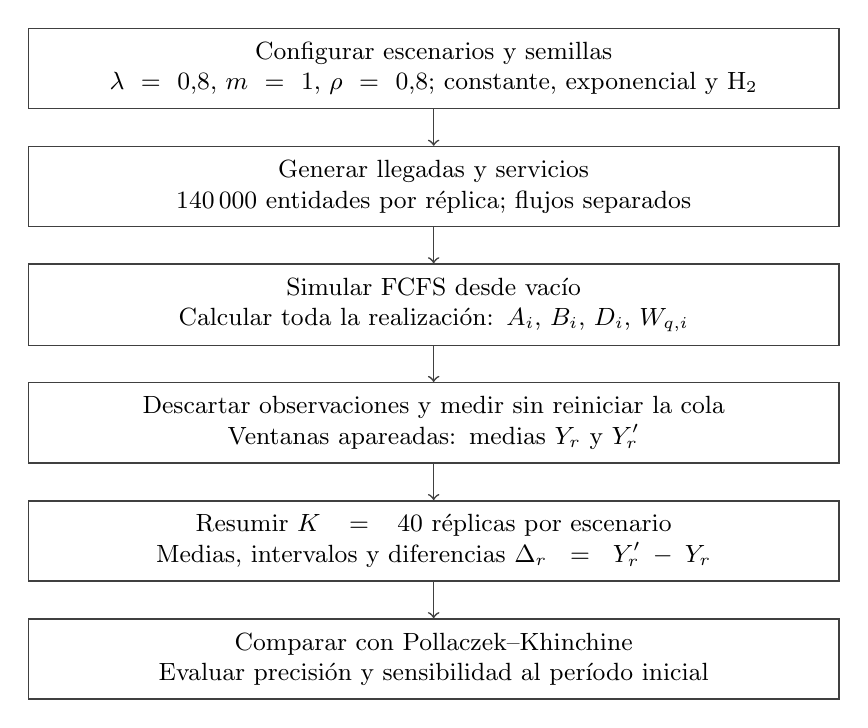
\begin{tikzpicture}[
  x=\textwidth,y=1cm,font=\small,
  etapa/.style={draw=black!75,fill=white,line width=0.5pt,
    text width=0.82\textwidth,align=center,inner sep=5pt,
    minimum height=0.95cm},
  flujo/.style={->,draw=black!75,line width=0.6pt}
]
  \node[etapa] (configuracion) at (0,0)
    {Configurar escenarios y semillas\\
     $\lambda=0{,}8$, $m=1$, $\rho=0{,}8$; constante, exponencial y H$_2$};
  \node[etapa] (generacion) at (0,-1.5)
    {Generar llegadas y servicios\\
     $140\,000$ entidades por réplica; flujos separados};
  \node[etapa] (simulacion) at (0,-3)
    {Simular FCFS desde vacío\\
     Calcular toda la realización: $A_i$, $B_i$, $D_i$, $W_{q,i}$};
  \node[etapa] (medicion) at (0,-4.5)
    {Descartar observaciones y medir sin reiniciar la cola\\
     Ventanas apareadas: medias $Y_r$ y $Y'_r$};
  \node[etapa] (resumen) at (0,-6)
    {Resumir $K=40$ réplicas por escenario\\
     Medias, intervalos y diferencias $\Delta_r=Y'_r-Y_r$};
  \node[etapa] (contraste) at (0,-7.5)
    {Comparar con Pollaczek--Khinchine\\
     Evaluar precisión y sensibilidad al período inicial};
  \draw[flujo] (configuracion.south) -- (generacion.north);
  \draw[flujo] (generacion.south) -- (simulacion.north);
  \draw[flujo] (simulacion.south) -- (medicion.north);
  \draw[flujo] (medicion.south) -- (resumen.north);
  \draw[flujo] (resumen.south) -- (contraste.north);
\end{tikzpicture}

  \caption{Esquema del procedimiento de simulación previsto, desde la configuración hasta el contraste analítico y el diagnóstico de inicialización. $Y_r$ y $Y'_r$ representan las medias de las ventanas principal y alternativa de una misma réplica. Elaboración propia: diseño previsto, no resultados ni software ya ejecutado.}
  \label{fig:procedimiento-simulacion}
\end{figure}

\subsection{Réplicas y reproducibilidad pseudoaleatoria}
\label{subsec:metodo-replicas}

Se realizarán $K=40$ réplicas independientes por escenario. Cada una generará $140\,000$ llegadas y servicios desde vacío. La estimación principal descartará las primeras $b=20\,000$ llegadas y utilizará las siguientes $n=100\,000$, índices $b+1,\ldots,b+n$. Descartar observaciones no reiniciará la cola: se conservarán el trabajo pendiente y la evolución acumulada. El sufijo adicional permitirá el diagnóstico de inicialización descrito más adelante. Se fija un presupuesto por cantidad de entidades, no por minutos simulados; estos valores son decisiones iniciales de diseño y no demuestran estacionariedad ni precisión suficiente.

La semilla maestra será 2026. Para cada escenario y réplica se construirá una \texttt{SeedSequence} de NumPy con los enteros \texttt{[2026, escenario, replica]}, donde los escenarios tendrán identificadores $0,1,2$ y las réplicas $0,\ldots,39$. Desde ella se derivarán mediante \texttt{spawn} flujos separados para intervalos de llegada, elección del componente y duraciones de servicio. Se mantendrá esta asignación incluso cuando un escenario no necesite elegir componentes. Se asumirá independencia práctica entre flujos pseudoaleatorios, no una garantía criptográfica. No se usarán números aleatorios comunes entre escenarios; el apareamiento se reservará al diagnóstico dentro de una misma realización.

\subsection{Estimación e incertidumbre estadística}
\label{subsec:metodo-inferencia}

La unidad del análisis estadístico será la media de cada réplica,
\begin{equation}
  Y_r=\frac{1}{n}\sum_{i=b+1}^{b+n}W_{q,i}^{(r)},\qquad
  \overline{Y}=\frac{1}{K}\sum_{r=1}^{K}Y_r,\qquad
  s_Y^2=\frac{\sum_{r=1}^{K}(Y_r-\overline{Y})^2}{K-1}.
  \label{eq:metodo-estimadores}
\end{equation}
Las esperas sucesivas dentro de una réplica pueden estar correlacionadas: no se tratarán como observaciones independientes para calcular el error estándar. El método de réplicas permite estimar la variabilidad entre medias, distinguiéndola de la dependencia interna \cite{banksAnalisisSalidas}. Se construirá el intervalo aproximado del $95\,\%$
\begin{equation}
  \overline{Y}\pm h,\qquad
  h=t_{0{,}975;K-1}\frac{s_Y}{\sqrt{K}},
  \label{eq:metodo-intervalo}
\end{equation}
donde $t_{0{,}975;K-1}$ es el cuantil de Student con $K-1$ grados de libertad. Su aproximación dependerá de la distribución de las medias de réplica. El intervalo describirá variabilidad Monte Carlo condicionada al modelo y al diseño, no sesgo residual, validez del modelo ni una cobertura exacta universal.

Se informará la semiamplitud relativa $h/\overline{Y}$, con meta diagnóstica de no superar el $5\,\%$. Si el presupuesto fijado no alcanzara esa precisión, se declarará la limitación, sin prolongar automáticamente las ejecuciones. También se calculará el error relativo $(\overline{Y}-w_\star)/w_\star$, donde $w_\star$ es la referencia analítica correspondiente. La inclusión de esa referencia en el intervalo será descriptiva: ni error exactamente nulo ni cobertura en toda ejecución serán requisitos de aprobación. La comparación principal será analítica; las simulaciones la ilustrarán, sin inferir diferencias entre modelos a partir del mero solapamiento de intervalos marginales.

\subsection{Sensibilidad al período inicial}
\label{subsec:metodo-inicializacion}

El inicio vacío puede introducir sesgo frente al régimen estacionario; aumentar las réplicas no lo elimina por sí mismo \cite{banksAnalisisSalidas}. Se evaluará una alternativa con descarte $b'=40\,000$ y las siguientes $100\,000$ llegadas de la \emph{misma} realización. Para cada réplica se obtendrá $Y'_r$ y la diferencia apareada $\Delta_r=Y'_r-Y_r$. Las ventanas se superpondrán, por lo que no serán independientes entre sí; las diferencias sí se analizarán como independientes entre réplicas.

La figura~\ref{fig:ventanas-medicion} sitúa ambas ventanas en un único eje de índices de entidad. El tramo común de medición comprende las entidades $40\,001$ a $120\,000$; las últimas $20\,000$ solo intervienen en la media alternativa. No habrá una segunda simulación ni un reinicio de estado al cambiar de ventana.

\begin{figure}[htbp]
  \centering
  % Fragmento editable: solo TikZ básico, sin bibliotecas adicionales.
% Escala común proporcional: x = índice / 140000.
% Límites exactos: 0, 1/7, 2/7, 6/7, 1.
% Las barras ocupan 0.84\textwidth; los extremos dejan margen para rótulos.
% Los descartes se rotulan fuera de los segmentos cortos, sin reducir letra.
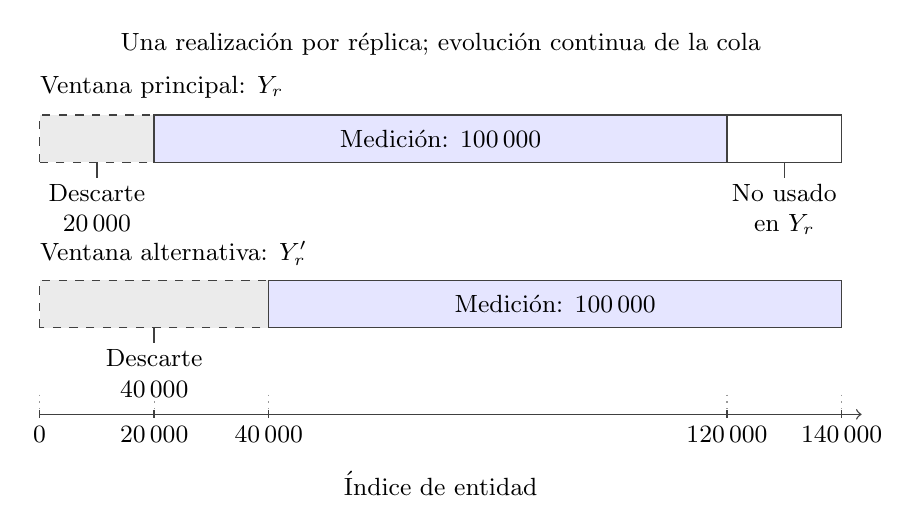
\begin{tikzpicture}[
  x=0.84\textwidth,y=1cm,font=\small,
  borde/.style={draw=black!75,line width=0.5pt},
  descarte/.style={borde,fill=black!8,dashed},
  medicion/.style={borde,fill=blue!10},
  nota/.style={align=center,inner sep=2pt}
]
  \node[nota] at (0.5,2.5)
    {Una realización por réplica; evolución continua de la cola};
  \node[anchor=west,inner sep=0pt] at (0,1.95) {Ventana principal: $Y_r$};
  \path[descarte] (0,1) rectangle ({1/7},1.6);
  \path[medicion] ({1/7},1) rectangle ({6/7},1.6);
  \path[borde,fill=white] ({6/7},1) rectangle (1,1.6);
  \node[nota] at (0.5,1.3) {Medición: $100\,000$};
  \draw[borde] ({1/14},1) -- ({1/14},0.8);
  \node[nota,anchor=north] at ({1/14},0.8) {Descarte\\$20\,000$};
  \draw[borde] ({13/14},1) -- ({13/14},0.8);
  \node[nota,anchor=north] at ({13/14},0.8) {No usado\\en $Y_r$};

  \node[anchor=west,inner sep=0pt] at (0,-0.15) {Ventana alternativa: $Y'_r$};
  \path[descarte] (0,-1.1) rectangle ({2/7},-0.5);
  \path[medicion] ({2/7},-1.1) rectangle (1,-0.5);
  \node[nota] at ({9/14},-0.8) {Medición: $100\,000$};
  \draw[borde] ({1/7},-1.1) -- ({1/7},-1.3);
  \node[nota,anchor=north] at ({1/7},-1.3) {Descarte\\$40\,000$};

  % Proyecciones de los límites sobre un único eje de índices, no temporal.
  \foreach \x in {0,{1/7},{2/7},{6/7},1} {
    \draw[draw=black!40,line width=0.45pt,dotted]
      (\x,-1.95) -- (\x,-2.2);
  }
  \draw[borde,->] (0,-2.2) -- (1.025,-2.2);
  \foreach \x/\valor in {0/0,{1/7}/{20\,000},{2/7}/{40\,000},
      {6/7}/{120\,000},1/{140\,000}} {
    \draw[borde] (\x,-2.15) -- (\x,-2.25);
    \node[anchor=north,inner sep=2pt] at (\x,-2.28) {$\valor$};
  }
  \node[nota,anchor=north] at (0.5,-2.85) {Índice de entidad};
\end{tikzpicture}

  \caption{Esquema de las ventanas apareadas sobre una misma realización de $140\,000$ entidades. Cada bloque delimitado por $a$ y $b$ comprende los índices $a+1,\ldots,b$; el eje cuenta entidades, no minutos. El descarte principal abarca $1$--$20\,000$ y la medición $20\,001$--$120\,000$; la alternativa descarta $1$--$40\,000$ y mide $40\,001$--$140\,000$. La cola evoluciona sin reinicios. Elaboración propia: diseño previsto y esquema del procedimiento, no resultados.}
  \label{fig:ventanas-medicion}
\end{figure}

Se calcularán $\overline{\Delta}$, su desviación muestral $s_\Delta$ y el intervalo aproximado $\overline{\Delta}\pm h_\Delta$, con $h_\Delta=t_{0{,}975;K-1}s_\Delta/\sqrt{K}$. Se usará el criterio práctico
\begin{equation}
  |\overline{\Delta}|+h_\Delta\leq 0{,}02\,w_\star.
  \label{eq:metodo-sensibilidad}
\end{equation}
Esta comprobación acotará la diferencia detectable respecto de un umbral propio del diseño; no probará ausencia de sesgo, pues ambas ventanas podrían compartirlo. Si no se satisficiera, se informará incertidumbre residual de inicialización, sin reintentos ilimitados ni declaración automática de convergencia. Los tamaños y umbrales propuestos no se atribuyen como recomendaciones numéricas de las diapositivas citadas.

\subsection{Verificación prevista y productos trazables}
\label{subsec:metodo-verificacion}

Antes de interpretar salidas, se incorporarán pruebas deterministas visibles y ejecutables desde el notebook. Con llegadas $A=[0;0{,}5;2]$ y servicios $S=[1;1;1]$, deberán obtenerse inicios $B=[0;1;2]$, salidas $D=[1;2;3]$ y esperas $[0;0{,}5;0]$. El caso $A=[0;2;4]$, con iguales servicios, deberá producir esperas nulas. Se comprobarán esperas no negativas, orden FCFS, ausencia de servicios superpuestos y la identidad $T_i=W_{q,i}+S_i$. Las medias y varianzas muestrales de entrada se contrastarán con sus momentos conocidos como diagnóstico, no exigiendo igualdad exacta.

Después se contrastarán medias estimadas, intervalos y errores con Pollaczek--Khinchine. Esta verificación de consistencia con un modelo conocido no validará un servicio real. Se conservarán CSV con configuración y métricas por réplica, y una tabla resumen con media, varianza entre réplicas, intervalo, referencia, error y diagnósticos de precisión e inicialización. El notebook, las semillas y las versiones permitirán reconstruir el procedimiento.

Se prepararán cuatro figuras complementarias: las funciones de distribución acumulada teóricas de los servicios, la espera media simulada con sus intervalos y referencias analíticas, la distribución acumulada descriptiva de las esperas y la sensibilidad al descarte inicial. La primera será analítica, con un salto en $m$ para el servicio constante; las demás se basarán en salidas efectivamente obtenidas. Para describir las esperas se acumularán, en la ventana principal de cada réplica, conteos en $321$ umbrales entre $0$ y $100m$. Se dividirá su suma por $Kn$ y se informará la fracción superior al último umbral. La curva entre umbrales será una representación discretizada, no la distribución empírica completa; no se supondrá independencia entre esperas ni se añadirán intervalos por observación. Este procesamiento descriptivo no cambiará los flujos aleatorios ni los estimadores principales.

El notebook incorpora una conexión explícita a Google Drive que requiere la autorización del usuario en Colab. Se creará una carpeta distinta por ejecución, con configuración y estado iniciales; las métricas y los conteos se guardarán tras cada réplica. Los archivos incompletos se identificarán como parciales y el estado solo indicará finalización después de exportar los productos. Las cuatro figuras se guardarán como PNG junto con sus datos CSV; no se exportará a PDF sin autorización. La versión anterior ejecutada por el usuario se conserva por separado. La ejecución integral, la persistencia en Drive y la revisión visual de la versión ampliada quedan pendientes de comprobación; su implementación no constituye por sí sola evidencia de resultados.
